\documentclass[12pt]{article}
\usepackage[utf8]{inputenc}
\usepackage{gettitlestring}
\usepackage{secdot}
\sectiondot{subsection}
\usepackage{geometry}
\geometry{a4paper,total={170mm,257mm},left=20mm,top=20mm,}
\usepackage{amsmath,amsfonts,amssymb,amsthm,braket,cancel,bigints,epsfig,epstopdf,titling,url,array, lastpage}
\usepackage[arrowdel,italicdiff]{physics}
\usepackage{hyperref, bookmark}
\usepackage{graphicx, wrapfig, subcaption, setspace, booktabs}
%\graphicspath{ {./%images/} }

\usepackage[myheadings]{fullpage}
\usepackage{fancyhdr}
\usepackage{float}
\usepackage{esint}
\usepackage[dvipsnames]{xcolor}
\usepackage{tikz}
\usepackage[font=small, labelfont=bf]{caption}
\usepackage[protrusion=true, expansion=true]{microtype}
\usepackage{sectsty}
\usepackage[spanish]{babel}
\usepackage{titling}
\usepackage{multirow}
\usepackage{csquotes}
\usepackage{xcolor}

\usepackage{caption}
\usepackage[nottoc]{tocbibind} %Adds "References" to the table of contents


% commands for including the picture
\newcommand{\titlepicture}[2][]{%
	\renewcommand\placetitlepicture{%
		\includegraphics[#1]{#2}\par\medskip
	}
}
\newcommand{\placetitlepicture}{} % initialization

\renewcommand{\contentsname}{Índice}
\renewcommand{\partname}{Parte}
\renewcommand{\figurename}{Figura}
\renewcommand{\tablename}{Tabla}

%\setcounter{section}{-1}


\newcommand{\HRule}[1]{\rule{\linewidth}{#1}}
\onehalfspacing
\setcounter{tocdepth}{5}
\setcounter{secnumdepth}{5}

%-------------------------------------------------------------------------------
% HEADER & FOOTER
%-------------------------------------------------------------------------------
\pagestyle{fancy}
\fancyhf{}
\setlength\headheight{15pt}
\fancyhead[L]{Machine Learning II}
\fancyhead[R]{Aprendizaje por refuerzo}
\fancyfoot[R]{Página \thepage\ de \pageref{LastPage}}
%-------------------------------------------------------------------------------
% TITLE PAGE
%-------------------------------------------------------------------------------

\begin{document}
	\title{ \large \textsc{\\[-2cm]Machine Learning II\\[0.5cm ]}
		\HRule{1pt} \\
		\LARGE \textbf{\uppercase{Aprendizaje por refuerzo}}\\
		[-0.5cm]\HRule{1pt} \\ 
		\large \textsc{\\Entorno Acrobot}
	}
	\author{\phantom{aaaaa}\\
		\phantom{aaa} \\
		\phantom{aaa} \\
		\phantom{aaa} \\
		\phantom{aaa} \\
		\phantom{aaa} \\
		\phantom{aaa} \\
		\phantom{aaa} \\
		\phantom{aaa} \\
		\phantom{aaa} \\
		\phantom{aaa} \\
		\phantom{aaa} \\
		Juan Miguel Ramos Pugnaire\\
		Andrés Canalejo Oliva\\
		Pablo Pérez González-Alberto\\
		Pablo Cardenal Real de Asúa
	}
	\newpage
	\begin{figure}[t!]
		\centering
		\phantom{aaaaa}\\[-3cm]
		
\includegraphics[width=0.4\linewidth]{Imagenes/logo.png}
	\end{figure}
	
	
	\maketitle
	
	\pdfbookmark[section]{\contentsname}{}
	\tableofcontents
	\newpage
	
	
	\section{Introducción}
	
	El aprendizaje por refuerzo (RL por sus siglas en inglés) se basa en la idea de que un agente aprende a tomar decisiones interactuando con un entorno. De esta forma, el agente aprende a maximizar una recompensa basada en sus acciones, lo que le permite aprender a realizar tareas complejas a través de la exploración del entorno y la adaptación a los cambios en él.
	
	En el presente trabajo, se utilizará RL para entrenar a un agente que controle el movimiento del robot \textit{Acrobot}, utilizando el paquete \texttt{gym} de OpenAI. 
	
	El entorno consiste en un robot de dos brazos que puede girar alrededor de su base. El robot se encuentra en un estado inicial colgando hacia abajo y debe alcanzar una posición objetivo que se define como el momento en que el extremo superior del segundo brazo del robot alcanza una altura específica. En la siguiente figura se representa la posición inicial del agente y la altura que debe alcanzar para obtener la recompensa:
	
	\begin{figure}[H]
		\centering
		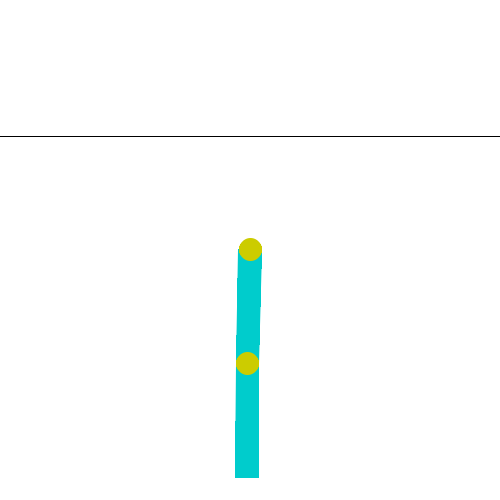
\includegraphics[width = 0.5\linewidth]{Imagenes/acrobot0.png}
		\caption{Posición inicial del robot controlado por el agente}
		\label{f:acrobot0}
	\end{figure}
	
	En lo que respecta al espacio de acciones y observaciones del agente, son de categoría discreta y continua respectivamente. Siguiendo la misma nomenclatura que la documentación, las acciones disponibles para el agente son las siguientes:
	\begin{itemize}
		\item Acción 0: Aplicar torque negativo a la primera articulación (-1)
		\item Acción 1: No aplicar torque (0)
		\item Acción 2: Aplicar torque positivo a la primera articulación (1)
	\end{itemize}
	Por otro lado, el entorno viene dado por un vector de seis dimensiones representando las posiciones y velocidades los eslabones del acrobot. Denominando $\theta_1$ al ángulo de la primera unión y $\theta_2$ al de la segunda, los parámetros del entorno son los siguientes
	\begin{itemize}
		\item $\cos{(\theta_1)}$
		\item $\sin{(\theta_1)}$
		\item $\cos{(\theta_2)}$
		\item $\sin{(\theta_2)}$
		\item $\dot{\theta_1}$: Velocidad angular de $\theta_1$ 
		\item $\dot{\theta_1}$: Velocidad angular de $\theta_2$
	\end{itemize}
	Las funciones trigonométricas toman valores entre $[-1,1]$, trivialmente, y las velocidades angulares varían entre $[-4\pi,4\pi]$ y $[-9\pi, 9\pi]$ para $\dot{\theta_1}$ y $\dot{\theta_2}$, respectivamente
	
	
	\section{Objetivos}
	
	El objetivo del trabajo es entrenar un agente que sea capaz de controlar con éxito el movimiento del robot y alcanzar la posición objetivo en el menor número de episodios posible. Además, se busca analizar y comparar la eficacia de los métodos seleccionados para resolver el problema y así identificar el método más eficiente para la tarea en cuestión.
	
	\section{Métodos seleccionados}
	
	La selección de los métodos de aprendizaje por refuerzo utilizados en este trabajo se basa en un análisis detallado del entorno Acrobot y en la adaptabilidad de los métodos de RL a este entorno en particular. En primer lugar, cabe destacar que debido al espacio de observaciones continuo no se puede usar Q-Learning y, por extensión, tampoco Double Q-Learning. Por otro lado, como el espacio de acciones es discreto también es necesario descartar DDPG y TD3 ya que ambos trabajan sobre un espacio continuo de acciones.
	
	Por tanto, los métodos escogidos para la resolución del problema son los siguientes:
	\begin{itemize}
		\item DQN es una buena opción ya que es una generalización de Q-learning que utiliza una red neuronal profunda para aproximar el valor de Q. Se ha demostrado que funciona bien en espacios de observaciones continuos como Acrobot, lo que lo convierte en una opción viable para nuestro problema.
		\item Double DQN es una mejora de DQN que ayuda a reducir la sobreestimación del valor de Q, lo que lo hace aún más efectivo en entornos complejos. Al igual que DQN, se ha demostrado que funciona bien en entornos continuos.
		\item  Reinforce es un método de gradiente de políticas que funciona bien en entornos con acciones continuas y puede ser útil para explorar diferentes estrategias de acción en Acrobot.
		
	\end{itemize}

	\subsection{Deep Q-Learning}
	
	\subsection{Double Deep Q-Learning}
	
	\subsection{Algoritmo REINFORCE}
	
		Para la realización del algoritmo se ha usado una red neuronal relativamente sencilla, de únicamente dos capas ocultas de 32 neuronas cada una. La función de activación se ha escogido como ReLU por sus buenos resultados en gran cantidad de problemas. LA capa de entrada es de 6 neuronas por ser el espacio de observaciones de 6 dimensiones y la capa final son 3 neuronas representando las tres acciones. Como es necesario que esta capa sea una distribución de probabilidad se necesita usar softmax como función de activación.
		
		En lo que respecta a la ejecución del programa se han definido dos funciones, \verb|play_one_step| y \verb|play_multiple_episodes|, acorde a la naturaleza del algoritmo. La primera función calcula el estado del entorno, la recompensa y los gradientes mientras que la segunda se usa para simular varios episodios. Los parámetros utilizados en el código son los siguientes:
		\begin{itemize}
			\item \verb|n_iterations|: Representa el número total de iteraciones o actualizaciones del agente. Cada iteración implica jugar múltiples episodios y realizar ajustes en el modelo de acuerdo con las recompensas obtenidas. Se ha tomado \verb|n_iterations = 125|
		
			\item \verb|n_episodes_per_update|: Indica el número de episodios jugados por cada actualización del modelo. Después de jugar estos episodios, se calculan las recompensas y los gradientes, y se ajustan los pesos del modelo en función de ellos. Se ha tomado \verb|n_episodes_per_update = 8|
		
			\item \verb|n_max_steps|: Es el número máximo de pasos que el agente jugará en cada episodio. Si el agente no ha terminado el episodio después de alcanzar este límite, se detendrá y se pasará al siguiente episodio. Se ha establecido \verb|n_max_steps|
		
			\item \verb|discount_rate|: Es el factor de descuento utilizado para calcular las recompensas descontadas. Determina el peso relativo de las recompensas pasadas y futuras en el proceso de aprendizaje del agente. En este caso, se establece en \verb|discount_rate = 0.99|, lo que significa que las recompensas futuras se descuentan en un 1\% por cada paso en el tiempo.
		\end{itemize}

		A la hora de entrenar el modelo hemos tenido bastantes problemas por la implementación seguida en clase. El código almacena en memoria todas las recompensas, lo que hace que conforme avance el entrenamiento esta se llene. La magnitud del problema es tal que el ordenador donde se ha entrenado el modelo, con 32 GB de RAM, ha sufrido apagados forzados. Para solucionarlo hemos decidido persistir en disco los valores de las recompensas y reiniciar el vector. Esto añade un poco de latencia al tener que abrir el archivo, escribir las recompensas y cerrarlo, pero podemos entrenar el modelo en una cantidad muy razonable de tiempo; especialmente comparado con los modelos anteriores.
		
		Los resultados de las recompensas se han representado en la siguiente figura:
		\begin{figure}[H]
			\centering
			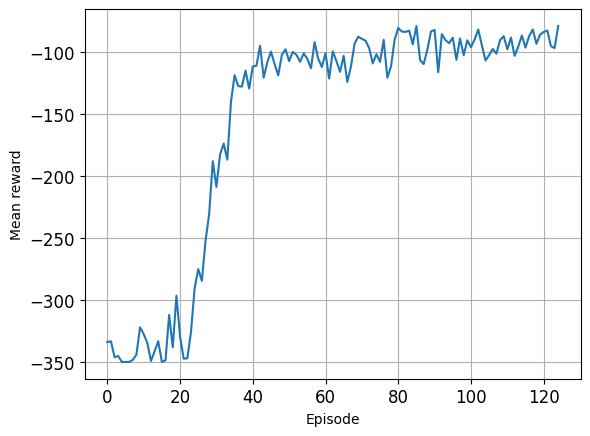
\includegraphics[width = 0.5\linewidth]{Imagenes/outputREINFORCE.png}
			\caption{Evolución de las recompensas a lo largo de las diferentes iteraciones para el algoritmo de REINFORCE.}
			\label{f:reinforce}
		\end{figure}
		Se observa una clara mejoría entre los episodios 20 y 40, pero a partir de esta iteración se estabiliza. El modelo sigue mejorando pero no al mismo ritmo que el intervalo anterior. Esto sugiere que el agente ha sido capaz de encontrar una política que le permita alcanzar recompensas de manera consistente. Eso se puede corroborar usando el vídeo adjunto a la memoria, en el que se ve que el agente es capaz de llegar sin problema a la meta.



\end{document}